\chapter{Liquid Argon Detectors at the Intensity Frontier}\label{ch:2}
In the next few years, LArTPC experiments -- such as the Short-Baseline Neutrino program (SBN) and DUNE -- will  be the tools to answer some of the burning questions in neutrino physics today.  This section illustrates the operational principles of this detector technology, as well as the scope of SBN, DUNE and LArIAT in the current intensity frontier panorama.


\section{The Liquid Argon Time Projection Chamber Technology}

\subsection{Time Projection Chamber}
\subsection{LArTPC: Principles of Operation}\label{sec:LArTPCWorkingPrinciple}

%The time projection chamber (TPC) was invented by Nygren in 1974 [91]. The proposal to implement a liquid argon TPC (LArTPC) for neutrino physics was made by Rubbia in 1977 [92], and the concept was implemented by the ICARUS collaboration [93]. 

To the bare bones, a LArTPC is a bulk of liquid argon sandwiched in a flat capacitor, equipped with a light collection system. A uniform electric field of the order of 500 V/cm is maintained constant between the faces of the capacitor. The anode is sensitive to ionization charge and it is usually made of two or more planes segmented into several hundreds parallel sense wires a few millimeters apart; different geometries for the anode segmentation are under study \cite{1748-0221-8-07-P07002}. 

Argon ionization and scintillation are the processes leveraged to detect particles in the LArTPC active volume.  When a ionizing radiation traverses the argon active volume it leaves a trail of ionization electrons along its trajectory and it excites the argon, leading to the production of scintillation light -- details on the production and detection of ionization charge and scintillation light are provided in \ref{sec:light} and \ref{sec:light} respectively. The optical part of the detector collects the argon scintillation light in matters of nanoseconds. This flash of light determines the start time of an event in the chamber, $t_0$. The uniform electric field drifts the ionization  electrons from the production point towards the anode plane in order of hundreds of microseconds or more depending on the chamber dimensions\footnote{The ionized argon also drifts, but  in the opposite directions compared to the electrons. Since the drift time is proportional to the particle mass,  the ions drift time is much longer than the electrons'.  Ionized argon is collected on the cathode which is not instrumented, so it is not used to infer information about the interactions in the chamber.}. The anode sense wires see either an induced current by the drifting charge (on induction planes) or an injection of the ionization charge (collection plane) [94].    An appropriate choice of the voltage bias on each wire plane assures ideal charge transparency, so that all the ionization charge is collected on the collection plane and none on the induction planes [95].  

The arrival time of the charge on the anode sense wires is used to measure the position of the original ionizing radiation in the drift direction. In fact, since the constant electric field implies that the drift velocity is also constant in the chamber, the position of the original ionization is simply given by the multiplication of the drift velocity by the drift time, where we define as ``drift time" the difference between $t_0$ and the charge arrival time on the wire planes. The spacial resolution on this dimension is limited by the time resolution of the electronics or by longitudinal diffusion of the electrons.
The spatial information on the different wire planes maps a bi-dimensional projection of the interaction pattern in the plane perpendicular to the drift direction. The spacial resolution on this dimension is limited by the transverse electron diffusion in argon and by the grain of the anode segmentation, i.e. the spacing between the wires in the sense planes [100].  The off-line combination of the 2-D information on the wire planes with the timing information allows for the 3D reconstruction of the event in the chamber.

 
Calorimetry  

\subsection{Liquid Argon: Ionization Charge}\label{sec:charge}
\subsubsection{Electron Life Time \& purity}
LArTPCs use  hermetically sealed and leak-checked vessels to abate the leakage and diffusion of contaminants into the system. The liquid argon filling of the volume occurs after the vessel is evacuated or purged with gaseous argon [205]  to reduce remaining gases in the volume. Even so, the construction of a pure tank of argon is unviable, as several sources of impurity remain.  In particular, impurities can come from the raw argon supply, the argon filtration system and from the outgassing from internal surfaces. Outgassing is a continuous diffusive process  producing contaminants, especially water, even after the vessel is sealed, particularly from materials in the ullage region\footnote{.  While the liquid argon low temperature reduces outgassing in the liquid, this process remains significant for absorptive material (such as plastic) above the surface of the liquid phase}.  Since research-grade argon comes from the industrial distillation of air, the impurities with the highest concentration are nitrogen, oxygen and water, generally maintained under the 1 part per million level by the vendor.  Even so, a higher level of purity is necessary to achieve a free electron life time usable in meter scale detectors. Thus, argon  is constantly  filtered in the cryogenic system, which reduce the oxygen and water contamination to less than 100 parts per trillion. The filtration system depends on the size and drift distance of the experiment and, for experiments on several meters scale, it includes an argon recirculation system.

\subsubsection{Space Charge Effect}
\subsubsection{Recombination Effect}

%%%%%%%%%%%%%%%%%%%%%%%%%%%%%%%%%%%%%%%%%%%%%%%%%%%%%%%%%%%%%%%
%%%%%%%%%%%%%%%%%%%%%                     Light Detection             %%%%%%%%%%%%%%%%%%%%%%%%
%%%%%%%%%%%%%%%%%%%%%%%%%%%%%%%%%%%%%%%%%%%%%%%%%%%%%%%%%%%%%%%
\subsection{Liquid Argon: Scintillation Light }\label{sec:light}
Liquid argon emits scintillation light at the passage of charged particles. LArTPCs  leverage this property to determine when the ionization charge begins to drift towards the anode plane. %Scintillation light can also be used for particle identification, as discussed in the next sections.

\subsubsection{Scintillation Process}
Scintillation light in argon peaks in the ultraviolet at a 128 nm, shown in comparison to Xenon and Kypton in Figure  [183]. The light yield collected by the optical detector depends on the argon purity, the electric field, the dE/dx and particle type, averaging at the tens of thousands of photons per MeV. 
The de-excitation of Rydberg dimers in the argon is responsible for the scintillation light. 
Rydberg dimers exist in two states:  singlets and a triplets. The time constant for the singlet radiative decay is 6 ns, resulting in a prompt component for the scintillation light. The decay of the triplet is delayed by intersystem crossing, producing a slow component with a time constant of $\sim$~1500 ns.  ``Self-trapped exciton luminescence" and  ``recombination luminescence" are the two processes responsible for the creation of the Rydberg dimers. In the first process, a charged particle excites an argon atom which becomes self-trapped in the surrounding bulk of argon,  forming a dimer; the dimer is in the singlet state 65\% of the times and in the triplet state 35\% of the times. In case of recombination luminescence, the charged particle transfers enough energy to ionize the argon. The argon ion forms a charged argon dimer state, which quickly recombines with the thermalized free electron cloud. Excimer states are produced in the recombination, roughly half in the singlet and half in the triplet state. The light yield dependency on the electric field, on the dE/dx and particle type derives from the role of free charge in the recombination luminescence process. The spacial separation between the argon ions and the free electron cloud depends on the electric field. On one hand, a strong electric field diminishes the recombination probability, leading to a smaller light yield; on the other, it increases the free charge drifting towards the anode plane. Hence, the amount of  measurable charge and light anti-correlates as a function of the electric field.  Ionizing particles in the argon modify the local density of both free electrons and ions depending on their dE/dx. Since the recombination rate is proportional to the square of the local ionization density, highly ionizing particles boost recombination and the subsequent light yield compared to MIPs.  The possibility to leverage this dependency for pulseshape-based particle identification has been shown in [186], [187].

\subsubsection{Effects Modifying the  Light Yield}
The production mechanism through emission from bound excimer states implies that argon is  transparent to its own scintillation light. In fact, the photons emitted from these metastable states are not energetic enough to re-excite the argon bulk, greatly suppressing absorption mechanisms. In a LArTPC however, several processes modify the light yield in between the location where light is produced and the optical detector. In a hypothetical pure tank of argon, Rayleigh scattering would be the most important processes modifying the light yield. Rayleigh scattering changes the path of light propagation in argon, prolonging the time between light production and detection.  The scattering length has been measured to be 66 cm [191] , shorter than the theoretical prediction of $\sim$~90 cm [190]; this value is short enough to be relevant for the current size of LArTPCs detectors. In fact, Rayleigh scattering worsen the resolution on $t_0$, the start time for charge drifting, and  alters the light directionality, complicating the matching between light and charge coming from the same object in case of multiple charged particles in the detector. 

Traces of impurities in argon such as oxygen, water and nitrogen  also affect the light yield, mainly  via absorption and quenching mechanisms. 
Absorption occurs as the interaction of a 128 nm photon directly with the impurity dissolved in the liquid argon.  Differently, quenching occurs as the interaction of an argon excimer and an impurity, where the excimer transfers its excitation to the impurity and  dissociates non-radiatively.  Given this mechanism, it is evident how quenching is both a function of the impurity concentrations and the excimer lifetime.  Since the triplet states live much longer than the singlet states,  quenching occurs mainly on triplet states, affecting primarily the slow component of the light,  reducing the scintillation yield and a shortening of the scintillation time constants.  

The stringent constraints for the electron life time limit the presence of oxygen and water to such a low level that both absorption and quenching on these impurity is not expected to be significant [210].   Contrarily, the nitrogen level is not bound by the electron life time constraints -- nitrogen being an inert gas, expensive to filter. Thus, nitrogen is often present at the level provided by the vendor. The effects of nitrogen on argon scintillation light have been studied in the WArP R\&D program and at several test stands.
The quenching process induced by nitrogen in liquid Ar has been measured to be proportional to the nitrogen concentration, with a rate constant of $\sim  0.11$ $\mu s^{-1}$ ppm$^{-1}$; appreciable decreasing in lifetime and relative amplitude of the slow component have been shown for contamination as high as a few ppm of nitrogen \cite{1748-0221-5-06-P06003}.
For a nitrogen  concentration of 2 parts per million,  typical of the current generation of LArTPC, the attenuation length due to nitrogen has been measured to be $\sim$30 meters \cite{1748-0221-8-07-P07011}. 



\subsubsection{Wavelength Shifting of LAr Scintillation Light}
Liquid argon scintillation light is invisible for most optical detectors deployed in LArTPC, such as cryogenic PMTs and SiPMs, since a wavelength of 128 nm is  generally too short to be absorbed from most in glasses, polymers and semiconductor materials. Research on prototype SiPMs absorbing directly VUV light and their deployment in noble gasses experiment is ongoing but not mature \cite{1748-0221-8-01-C01003}. Thus, experiments need to shift the wavelength of scintillation light to be able to detect it.  Albeit deployed in different ways, neutrinos and dark matter experiments commonly use  1,1,4,4-tetraphenyl-butadiene (TPB) to shift the scintillation light. 
TPB, whose chemical structure is shown in figure , absorbs the vacuum ultraviolet (VUV) light and emits in the visible at $\sim$~425 nm [231], with a ratio of visible photon emitted per VUV photon absorbed of $\sim$1.2:1 \cite{GEHMAN2011116}.

Neutrino experiments typically coat their optical detector system evaporating a layer of TPB either directly on the PMTs glass surface or on acrylic plates mounted in front of the PMTs \textcolor{red}{cite microboone}; this technique allows the fast detection light coming directly from the neutrino interaction. Dark matter experiments typically evaporate TPB on reflective foils mounted on the inside walls of the sensitive volume and detect the light after it has been reflected; this technique leads to a higher and more uniform light yield, though scattering effects for both the visible and VUV light augment the propagation time and hinder directionality information\textcolor{red}{some DM detector} . In order to take advantage of both these techniques, hybrid systems with PMT coating and foils are being considered for the next generation of large neutrino detectors \textcolor{red}{cite SBND?}. 

\subsection{Signal processing}

\section{The Intensity Frontier Program}
\subsection{SBN: Neutrino Interaction and Detection}
%\subsection{SBN Goals}
%\subsection{Neutrino Interactions and Detection }
\subsection{DUNE: Rare Decay Searches}
The key elements for a rare decay experiment are: massive active volume, long exposure, high identification efficiency and low background. 
%The limit to proton lifetime in case of absence of signal and backgrounds is set by calculating
%$$\tau/B > M\times \epsilon\times T \times 10^{32},$$ 
%where M is the detector mass in kton, $\epsilon$ the signal detection efficiency after cuts to suppress backgrounds (dependent on the considered decay mode), T is the exposure in years, B the assumed branching fraction for the considered mode and  $10^{32}$ is a factor accounting for the number of nucleons in a kton of material \cite{Bueno2007}.
Figure \ref{fig:PDKExperimentalLImit} shows the current best experimental limits on nucleon decay lifetime over branching ratio (dots). Historically, the dominant technology used in these searches has been water Cherenkov detectors: all the best experimental limits on every decay mode are indeed set by Super-Kamiokande \cite{PhysRevD.90.072005,PhysRevLett.115.121803}.  It is particularly important to notice that the kaon energy for the proton decay mode $p \rightarrow K^+ \bar{\nu}$ is under Cherenkov threshold.  Super-Kamiokande set the limit on the lifetime for the $p \rightarrow K^+ \bar{\nu}$ mode by  relying exclusively on photons from nuclear de-excitation. For this reason, an attractive alternative approach to identifying nucleon decay is the use of a Liquid Argon Time Projection Chamber (LArTPC). 

LArTPCs can complement nucleon decay searches in modes where water Cherenkov detectors are less sensitive, especially $p\rightarrow K^+\bar{\nu}$. According to \cite{Acciarri:Dune}, DUNE will have an active volume large enough, have sufficient shielding from the surface, and will run for lengths of time sufficient to compete with Hyper-K, opening up the opportunity for the discovery of nucleon decay. 

\begin{figure}[hbpt]
\centering
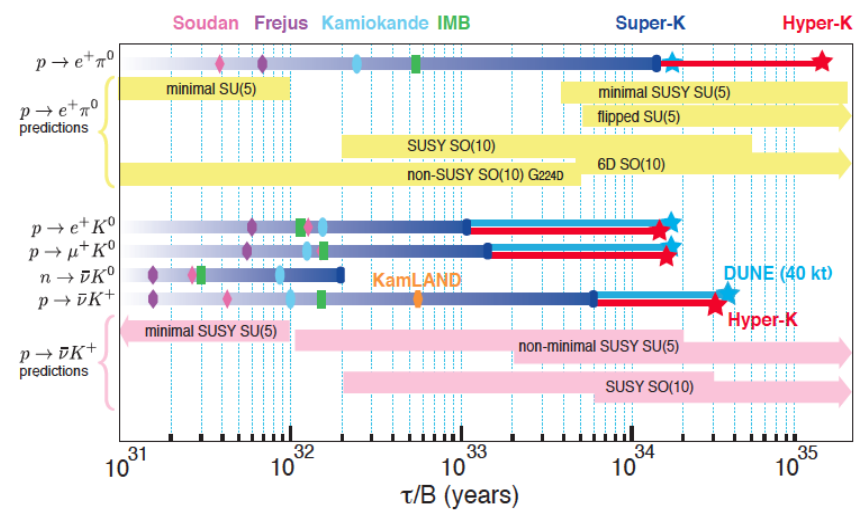
\includegraphics[width=6.5in]{Chapter-2/Images/PDKExperimentalLImit.png}
\caption{Proton decay lifetime limits from passed and future experiments.}
\label{fig:PDKExperimentalLImit}
\end{figure}


\begin{figure}[hbpt]
\centering
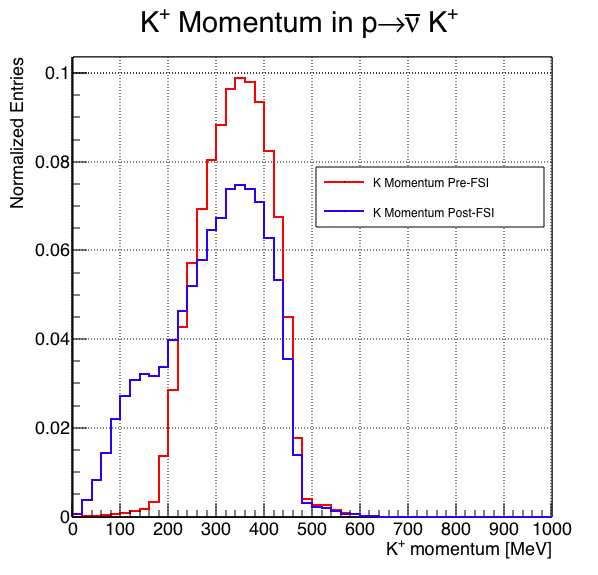
\includegraphics[width=3.5in]{Chapter-2/Images/pdkGenie.png}
\caption{Momentum of the kaon outgoing a proton decay event as simulated by the Genie 2.8.10 event generator in argon. The red line represent the kaon momentum distribution before undergoing the simulated final state interaction inside the argon nucleus, while the blue line represents the momentum distribution after FSI. }
\label{fig:PDKGENIE}
\end{figure}


%\subsection{Non-Accelerator Physics Program}
%\subsection{Rare Decay Searches: Experimental Limit}
%\subsection{Nucleon Decay Detection in LAr}
\subsection{Enabling the next generation of discoveries: LArIAT}
LArIAT, a small Liquid Argon Time Projection Chamber (LArTPC) in a test beam,  is designed to perform an extensive physics campaign centered on charged particle cross section measurements while characterizing the detector performance for future LArTPCs. LArTPC represents one of the most advanced experimental technologies for physics at the Intensity Frontier due to its full 3D-imaging, excellent particle identification and precise calorimetric energy reconstruction. This complex technology however needs a thorough calibration and dedicated measurements of some key quantities to achieve the precision required for the next generation of discoveries at the Intensity Frontier which LArIAT can provide. 

The LArIAT LArTPC is deployed in a dedicated calibration test beamline at Fermilab.
We use the LArIAT beamline to characterize the charge particles before they enter the TPC: the particle type and initial momentum is known from beamline information. The precise calorimetric energy reconstruction of the LArTPC technology enables the measurement of the total differential cross section for  tagged hadrons. 
The Pion-Nucleus and Kaon-Nucleus total hadronic interaction cross section have never been measured before in argon and they are a fundamental step to shed light on light meson interaction in nuclei. Additionally, these measures provides a key input to neutrino physics and proton decay studies in future LArTPC experiments like SBN and DUNE.
\textcolor{red}{add paragraph on all wonderful things lariat can do... some event displays would be nice!}



\textcolor{red}{ADD genie proton decay kaon distribution and lariat beamline overlaied}
The signature of a proton decay event in the ``LAr golden mode" is the presence of a single kaon of about 400 MeV in the detector. 
